% Options for packages loaded elsewhere
\PassOptionsToPackage{unicode}{hyperref}
\PassOptionsToPackage{hyphens}{url}
%
\documentclass[
  11pt,
  ignorenonframetext,
]{beamer}
\usepackage{pgfpages}
\setbeamertemplate{caption}[numbered]
\setbeamertemplate{caption label separator}{: }
\setbeamercolor{caption name}{fg=normal text.fg}
\beamertemplatenavigationsymbolsempty
% Prevent slide breaks in the middle of a paragraph
\widowpenalties 1 10000
\raggedbottom
\setbeamertemplate{part page}{
  \centering
  \begin{beamercolorbox}[sep=16pt,center]{part title}
    \usebeamerfont{part title}\insertpart\par
  \end{beamercolorbox}
}
\setbeamertemplate{section page}{
  \centering
  \begin{beamercolorbox}[sep=12pt,center]{part title}
    \usebeamerfont{section title}\insertsection\par
  \end{beamercolorbox}
}
\setbeamertemplate{subsection page}{
  \centering
  \begin{beamercolorbox}[sep=8pt,center]{part title}
    \usebeamerfont{subsection title}\insertsubsection\par
  \end{beamercolorbox}
}
\AtBeginPart{
  \frame{\partpage}
}
\AtBeginSection{
  \ifbibliography
  \else
    \frame{\sectionpage}
  \fi
}
\AtBeginSubsection{
  \frame{\subsectionpage}
}
\usepackage{amsmath,amssymb}
\usepackage{iftex}
\ifPDFTeX
  \usepackage[T1]{fontenc}
  \usepackage[utf8]{inputenc}
  \usepackage{textcomp} % provide euro and other symbols
\else % if luatex or xetex
  \usepackage{unicode-math} % this also loads fontspec
  \defaultfontfeatures{Scale=MatchLowercase}
  \defaultfontfeatures[\rmfamily]{Ligatures=TeX,Scale=1}
\fi
\usepackage{lmodern}
\usetheme[]{metropolis}
\ifPDFTeX\else
  % xetex/luatex font selection
\fi
% Use upquote if available, for straight quotes in verbatim environments
\IfFileExists{upquote.sty}{\usepackage{upquote}}{}
\IfFileExists{microtype.sty}{% use microtype if available
  \usepackage[]{microtype}
  \UseMicrotypeSet[protrusion]{basicmath} % disable protrusion for tt fonts
}{}
\makeatletter
\@ifundefined{KOMAClassName}{% if non-KOMA class
  \IfFileExists{parskip.sty}{%
    \usepackage{parskip}
  }{% else
    \setlength{\parindent}{0pt}
    \setlength{\parskip}{6pt plus 2pt minus 1pt}}
}{% if KOMA class
  \KOMAoptions{parskip=half}}
\makeatother
\usepackage{xcolor}
\newif\ifbibliography
\usepackage{color}
\usepackage{fancyvrb}
\newcommand{\VerbBar}{|}
\newcommand{\VERB}{\Verb[commandchars=\\\{\}]}
\DefineVerbatimEnvironment{Highlighting}{Verbatim}{commandchars=\\\{\}}
% Add ',fontsize=\small' for more characters per line
\newenvironment{Shaded}{}{}
\newcommand{\AlertTok}[1]{\textcolor[rgb]{1.00,0.00,0.00}{\textbf{#1}}}
\newcommand{\AnnotationTok}[1]{\textcolor[rgb]{0.38,0.63,0.69}{\textbf{\textit{#1}}}}
\newcommand{\AttributeTok}[1]{\textcolor[rgb]{0.49,0.56,0.16}{#1}}
\newcommand{\BaseNTok}[1]{\textcolor[rgb]{0.25,0.63,0.44}{#1}}
\newcommand{\BuiltInTok}[1]{\textcolor[rgb]{0.00,0.50,0.00}{#1}}
\newcommand{\CharTok}[1]{\textcolor[rgb]{0.25,0.44,0.63}{#1}}
\newcommand{\CommentTok}[1]{\textcolor[rgb]{0.38,0.63,0.69}{\textit{#1}}}
\newcommand{\CommentVarTok}[1]{\textcolor[rgb]{0.38,0.63,0.69}{\textbf{\textit{#1}}}}
\newcommand{\ConstantTok}[1]{\textcolor[rgb]{0.53,0.00,0.00}{#1}}
\newcommand{\ControlFlowTok}[1]{\textcolor[rgb]{0.00,0.44,0.13}{\textbf{#1}}}
\newcommand{\DataTypeTok}[1]{\textcolor[rgb]{0.56,0.13,0.00}{#1}}
\newcommand{\DecValTok}[1]{\textcolor[rgb]{0.25,0.63,0.44}{#1}}
\newcommand{\DocumentationTok}[1]{\textcolor[rgb]{0.73,0.13,0.13}{\textit{#1}}}
\newcommand{\ErrorTok}[1]{\textcolor[rgb]{1.00,0.00,0.00}{\textbf{#1}}}
\newcommand{\ExtensionTok}[1]{#1}
\newcommand{\FloatTok}[1]{\textcolor[rgb]{0.25,0.63,0.44}{#1}}
\newcommand{\FunctionTok}[1]{\textcolor[rgb]{0.02,0.16,0.49}{#1}}
\newcommand{\ImportTok}[1]{\textcolor[rgb]{0.00,0.50,0.00}{\textbf{#1}}}
\newcommand{\InformationTok}[1]{\textcolor[rgb]{0.38,0.63,0.69}{\textbf{\textit{#1}}}}
\newcommand{\KeywordTok}[1]{\textcolor[rgb]{0.00,0.44,0.13}{\textbf{#1}}}
\newcommand{\NormalTok}[1]{#1}
\newcommand{\OperatorTok}[1]{\textcolor[rgb]{0.40,0.40,0.40}{#1}}
\newcommand{\OtherTok}[1]{\textcolor[rgb]{0.00,0.44,0.13}{#1}}
\newcommand{\PreprocessorTok}[1]{\textcolor[rgb]{0.74,0.48,0.00}{#1}}
\newcommand{\RegionMarkerTok}[1]{#1}
\newcommand{\SpecialCharTok}[1]{\textcolor[rgb]{0.25,0.44,0.63}{#1}}
\newcommand{\SpecialStringTok}[1]{\textcolor[rgb]{0.73,0.40,0.53}{#1}}
\newcommand{\StringTok}[1]{\textcolor[rgb]{0.25,0.44,0.63}{#1}}
\newcommand{\VariableTok}[1]{\textcolor[rgb]{0.10,0.09,0.49}{#1}}
\newcommand{\VerbatimStringTok}[1]{\textcolor[rgb]{0.25,0.44,0.63}{#1}}
\newcommand{\WarningTok}[1]{\textcolor[rgb]{0.38,0.63,0.69}{\textbf{\textit{#1}}}}
\usepackage{longtable,booktabs,array}
\usepackage{calc} % for calculating minipage widths
\usepackage{caption}
% Make caption package work with longtable
\makeatletter
\def\fnum@table{\tablename~\thetable}
\makeatother
\usepackage{graphicx}
\makeatletter
\def\maxwidth{\ifdim\Gin@nat@width>\linewidth\linewidth\else\Gin@nat@width\fi}
\def\maxheight{\ifdim\Gin@nat@height>\textheight\textheight\else\Gin@nat@height\fi}
\makeatother
% Scale images if necessary, so that they will not overflow the page
% margins by default, and it is still possible to overwrite the defaults
% using explicit options in \includegraphics[width, height, ...]{}
\setkeys{Gin}{width=\maxwidth,height=\maxheight,keepaspectratio}
% Set default figure placement to htbp
\makeatletter
\def\fps@figure{htbp}
\makeatother
\setlength{\emergencystretch}{3em} % prevent overfull lines
\providecommand{\tightlist}{%
  \setlength{\itemsep}{0pt}\setlength{\parskip}{0pt}}
\setcounter{secnumdepth}{-\maxdimen} % remove section numbering
\ifLuaTeX
  \usepackage{selnolig}  % disable illegal ligatures
\fi
\IfFileExists{bookmark.sty}{\usepackage{bookmark}}{\usepackage{hyperref}}
\IfFileExists{xurl.sty}{\usepackage{xurl}}{} % add URL line breaks if available
\urlstyle{same}
\hypersetup{
  pdftitle={Análisis de presencias con procesos de puntos},
  pdfauthor={Gerardo Martín},
  hidelinks,
  pdfcreator={LaTeX via pandoc}}

\title{Análisis de presencias con procesos de puntos}
\subtitle{Tutorial intermedio de spatstat}
\author{Gerardo Martín}
\date{2022-06-29}

\begin{document}
\frame{\titlepage}

\hypertarget{simulaciuxf3n-de-presencias}{%
\section{Simulación de presencias}\label{simulaciuxf3n-de-presencias}}

\begin{frame}{Especificación de un centroide}
\protect\hypertarget{especificaciuxf3n-de-un-centroide}{}
\begin{center}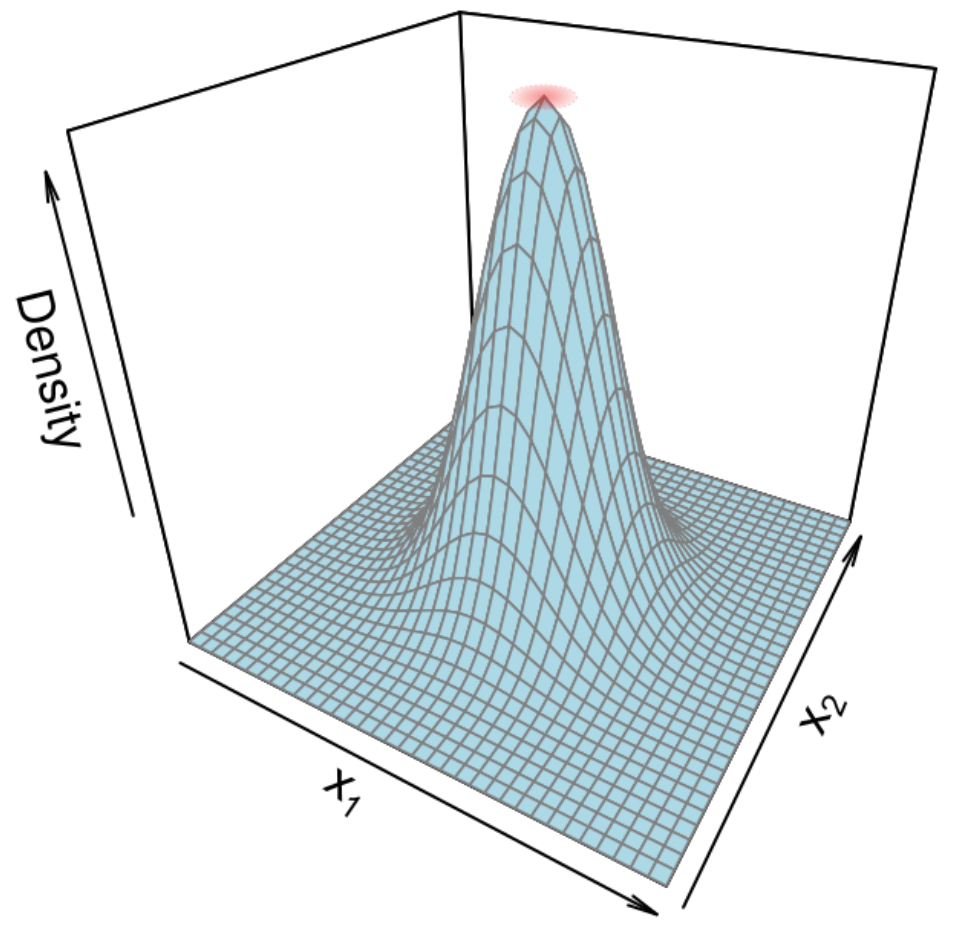
\includegraphics[width=13.28in]{Figuras/Centroide} \end{center}

\begin{itemize}
\tightlist
\item
  Abundancia alcanza un máximo y disminuye
\item
  Modelos más complicados con varias variables
\end{itemize}
\end{frame}

\begin{frame}[fragile]{Código - generando favorabilidad ``verdadera''}
\protect\hypertarget{cuxf3digo---generando-favorabilidad-verdadera}{}
\begin{Shaded}
\begin{Highlighting}[]
\NormalTok{centroide }\OtherTok{\textless{}{-}} \FunctionTok{global}\NormalTok{(r, mean)}
\NormalTok{r.df }\OtherTok{\textless{}{-}} \FunctionTok{as.data.frame}\NormalTok{(r, }\AttributeTok{xy =}\NormalTok{ T)}
\NormalTok{covar }\OtherTok{\textless{}{-}} \FunctionTok{cov}\NormalTok{(r.df[, }\DecValTok{3}\SpecialCharTok{:}\DecValTok{5}\NormalTok{])}
\NormalTok{md }\OtherTok{\textless{}{-}} \FunctionTok{mahalanobis}\NormalTok{(r.df[, }\DecValTok{3}\SpecialCharTok{:}\DecValTok{5}\NormalTok{], }\AttributeTok{center =}\NormalTok{ centroide}\SpecialCharTok{$}\NormalTok{mean, }\AttributeTok{cov =}\NormalTok{ covar)}
\FunctionTok{head}\NormalTok{(md)}
\end{Highlighting}
\end{Shaded}

\begin{verbatim}
##        1        2        3        4        5        6 
## 5.846738 6.383437 6.443874 7.296541 6.475630 6.066614
\end{verbatim}
\end{frame}

\begin{frame}[fragile]{Código - viendo la favorabilidad}
\protect\hypertarget{cuxf3digo---viendo-la-favorabilidad}{}
\begin{Shaded}
\begin{Highlighting}[]
\NormalTok{md.r }\OtherTok{\textless{}{-}} \FunctionTok{rast}\NormalTok{(}\FunctionTok{data.frame}\NormalTok{(r.df[, }\DecValTok{1}\SpecialCharTok{:}\DecValTok{2}\NormalTok{], md))}
\NormalTok{md.exp }\OtherTok{\textless{}{-}} \FunctionTok{exp}\NormalTok{(}\SpecialCharTok{{-}}\FloatTok{0.5}\SpecialCharTok{*}\NormalTok{md.r)}
\FunctionTok{plot}\NormalTok{(md.exp)}
\end{Highlighting}
\end{Shaded}

\begin{center}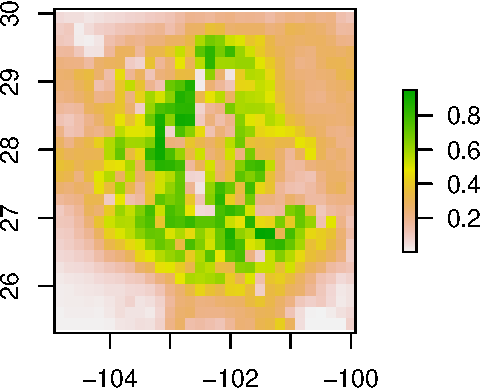
\includegraphics{Tutorial-spatstat-2_files/figure-beamer/unnamed-chunk-4-1} \end{center}
\end{frame}

\begin{frame}[fragile]{Código - simulando los puntos}
\protect\hypertarget{cuxf3digo---simulando-los-puntos}{}
\begin{Shaded}
\begin{Highlighting}[]
\FunctionTok{set.seed}\NormalTok{(}\DecValTok{182}\NormalTok{)}
\NormalTok{sam }\OtherTok{\textless{}{-}} \FunctionTok{sample}\NormalTok{(}\DecValTok{1}\SpecialCharTok{:}\FunctionTok{nrow}\NormalTok{(r.df), }\DecValTok{200}\NormalTok{, }\AttributeTok{prob =} \FunctionTok{exp}\NormalTok{(}\SpecialCharTok{{-}}\FloatTok{0.5}\SpecialCharTok{*}\NormalTok{md))}
\NormalTok{puntos}\FloatTok{.2} \OtherTok{\textless{}{-}} \FunctionTok{data.frame}\NormalTok{(r.df[, }\DecValTok{1}\SpecialCharTok{:}\DecValTok{2}\NormalTok{][sam,])}
\NormalTok{puntos}\FloatTok{.2}\SpecialCharTok{$}\NormalTok{x }\OtherTok{\textless{}{-}}\NormalTok{ puntos}\FloatTok{.2}\SpecialCharTok{$}\NormalTok{x }\SpecialCharTok{+} \FunctionTok{rnorm}\NormalTok{(}\DecValTok{200}\NormalTok{, }\DecValTok{0}\NormalTok{, }\FloatTok{0.05}\NormalTok{)}
\NormalTok{puntos}\FloatTok{.2}\SpecialCharTok{$}\NormalTok{y }\OtherTok{\textless{}{-}}\NormalTok{ puntos}\FloatTok{.2}\SpecialCharTok{$}\NormalTok{y }\SpecialCharTok{+} \FunctionTok{rnorm}\NormalTok{(}\DecValTok{200}\NormalTok{, }\DecValTok{0}\NormalTok{, }\FloatTok{0.05}\NormalTok{)}
\end{Highlighting}
\end{Shaded}
\end{frame}

\begin{frame}[fragile]{Código - favorabilidad y puntos}
\protect\hypertarget{cuxf3digo---favorabilidad-y-puntos}{}
\begin{Shaded}
\begin{Highlighting}[]
\FunctionTok{plot}\NormalTok{(md.exp); }\FunctionTok{points}\NormalTok{(puntos}\FloatTok{.2}\NormalTok{)}
\end{Highlighting}
\end{Shaded}

\begin{center}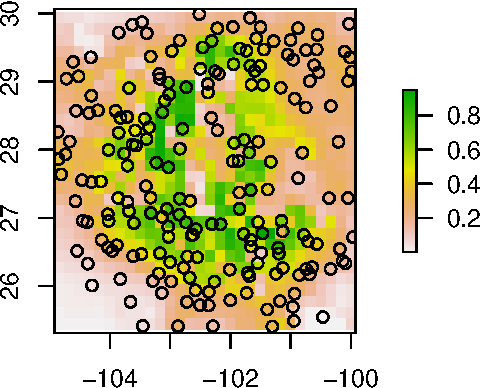
\includegraphics{Tutorial-spatstat-2_files/figure-beamer/unnamed-chunk-6-1} \end{center}
\end{frame}

\hypertarget{formateo-para-spatstat}{%
\section{Formateo para spatstat}\label{formateo-para-spatstat}}

\begin{frame}[fragile]{Cargando las funciones}
\protect\hypertarget{cargando-las-funciones}{}
\begin{Shaded}
\begin{Highlighting}[]
\FunctionTok{source}\NormalTok{(}\StringTok{"Funciones{-}spatstat/imFromStack.R"}\NormalTok{)}
\FunctionTok{source}\NormalTok{(}\StringTok{"Funciones{-}spatstat/winFromRaster.R"}\NormalTok{)}
\FunctionTok{source}\NormalTok{(}\StringTok{"Funciones{-}spatstat/plotQuantIntens.R"}\NormalTok{)}
\end{Highlighting}
\end{Shaded}
\end{frame}

\begin{frame}[fragile]{Formateo rápido}
\protect\hypertarget{formateo-ruxe1pido}{}
\begin{Shaded}
\begin{Highlighting}[]
\NormalTok{r.im }\OtherTok{\textless{}{-}} \FunctionTok{imFromStack}\NormalTok{(r)}
\FunctionTok{names}\NormalTok{(r.im) }\OtherTok{\textless{}{-}} \FunctionTok{paste}\NormalTok{(}\StringTok{"Var"}\NormalTok{, }\DecValTok{1}\SpecialCharTok{:}\DecValTok{3}\NormalTok{, }\AttributeTok{sep =} \StringTok{"."}\NormalTok{)}
\NormalTok{w }\OtherTok{\textless{}{-}} \FunctionTok{as.owin}\NormalTok{(r.im[[}\DecValTok{1}\NormalTok{]])}
\NormalTok{puntos.}\FloatTok{2.}\NormalTok{ppp }\OtherTok{\textless{}{-}} \FunctionTok{ppp}\NormalTok{(}\AttributeTok{x =}\NormalTok{ puntos}\FloatTok{.2}\SpecialCharTok{$}\NormalTok{x,}
                  \AttributeTok{y =}\NormalTok{ puntos}\FloatTok{.2}\SpecialCharTok{$}\NormalTok{y,}
                  \AttributeTok{window =}\NormalTok{ w,}
                  \AttributeTok{check =}\NormalTok{ F)}
\NormalTok{Q }\OtherTok{\textless{}{-}} \FunctionTok{pixelquad}\NormalTok{(}\AttributeTok{X =}\NormalTok{ puntos.}\FloatTok{2.}\NormalTok{ppp, }\AttributeTok{W =} \FunctionTok{as.owin}\NormalTok{(w))}
\end{Highlighting}
\end{Shaded}
\end{frame}

\hypertarget{anuxe1lisis-exploratorio}{%
\section{Análisis exploratorio}\label{anuxe1lisis-exploratorio}}

\begin{frame}[fragile]{Autocorrelación}
\protect\hypertarget{autocorrelaciuxf3n}{}
\begin{Shaded}
\begin{Highlighting}[]
\NormalTok{K }\OtherTok{\textless{}{-}} \FunctionTok{envelope}\NormalTok{(puntos.}\FloatTok{2.}\NormalTok{ppp, }\AttributeTok{fun =}\NormalTok{ Kest, }\AttributeTok{nsim =} \DecValTok{39}\NormalTok{)}
\end{Highlighting}
\end{Shaded}

\begin{verbatim}
## Generating 39 simulations of CSR  ...
## 1, 2, 3, 4, 5, 6, 7, 8, 9, 10, 11, 12, 13, 14, 15, 16, 17, 18, 19, 20,
## 21, 22, 23, 24, 25, 26, 27, 28, 29, 30, 31, 32, 33, 34, 35, 36, 37, 38, 
## 39.
## 
## Done.
\end{verbatim}
\end{frame}

\begin{frame}{Autocorrelación}
\protect\hypertarget{autocorrelaciuxf3n-1}{}
\begin{center}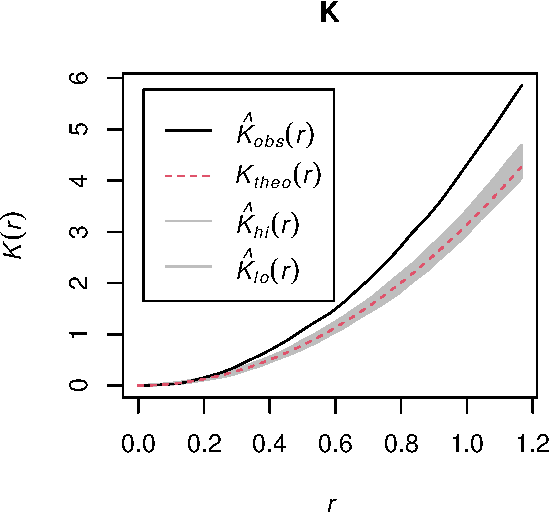
\includegraphics{Tutorial-spatstat-2_files/figure-beamer/unnamed-chunk-10-1} \end{center}
\end{frame}

\begin{frame}{Autocorrelación - notas}
\protect\hypertarget{autocorrelaciuxf3n---notas}{}
\begin{enumerate}
\tightlist
\item
  Pareciera que el proceso está levemente autocorrelacionado
\item
  No sabemos de momento si afectará al modelo
\item
  Debemos poner atención al modelo ajustado
\end{enumerate}
\end{frame}

\begin{frame}[fragile]{Respuestas a variables}
\protect\hypertarget{respuestas-a-variables}{}
\begin{Shaded}
\begin{Highlighting}[]
\FunctionTok{plotQuantIntens}\NormalTok{(}\AttributeTok{imList =}\NormalTok{ r.im,}
                \AttributeTok{noCuts =} \DecValTok{5}\NormalTok{,}
                \AttributeTok{Quad =}\NormalTok{ Q,}
                \AttributeTok{p.pp =}\NormalTok{ puntos.}\FloatTok{2.}\NormalTok{ppp,}
                \AttributeTok{dir =} \StringTok{""}\NormalTok{,}
                \AttributeTok{name =} \StringTok{"Respuestas{-}centroide"}\NormalTok{)}
\end{Highlighting}
\end{Shaded}

\begin{verbatim}
## pdf 
##   2
\end{verbatim}

\href{Respuestas-centroide.pdf}{Ver archivo de gráficas}
\end{frame}

\begin{frame}[fragile]{Consideraciones para proponer modelos}
\protect\hypertarget{consideraciones-para-proponer-modelos}{}
Curvas con forma de campana \(\rightarrow\) fórmula cuadrática

\begin{Shaded}
\begin{Highlighting}[]
\FunctionTok{curve}\NormalTok{(}\FunctionTok{exp}\NormalTok{(}\DecValTok{1} \SpecialCharTok{+}\NormalTok{ x }\SpecialCharTok{{-}}\NormalTok{ x}\SpecialCharTok{\^{}}\DecValTok{2}\NormalTok{), }\AttributeTok{from =} \SpecialCharTok{{-}}\DecValTok{3}\NormalTok{, }\DecValTok{3}\NormalTok{)}
\end{Highlighting}
\end{Shaded}

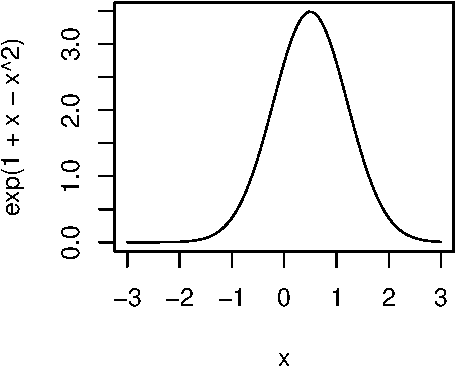
\includegraphics{Tutorial-spatstat-2_files/figure-beamer/unnamed-chunk-12-1.pdf}
\end{frame}

\begin{frame}{Consideraciones para proponer modelos}
\protect\hypertarget{consideraciones-para-proponer-modelos-1}{}
Ecuación lineal:

\[ y = \alpha + \beta_1 x_1 + \dots + \beta_n x_n\] Ecuación polinomial
de 2\(^o\) grado

\[ y = \alpha + \beta_1 x_1 + \beta_1' x_1^2 + \dots + \beta_n x_n + \beta_n' x_n^2\]
Recordemos que \(y = \log \lambda\)
\end{frame}

\begin{frame}[fragile]{¿Qué variables podemos incluir en el mismo
modelo?}
\protect\hypertarget{quuxe9-variables-podemos-incluir-en-el-mismo-modelo}{}
\textbf{Regla de oro}: Aquellas que no estén correlacionadas

\begin{itemize}
\tightlist
\item
  Que \(x_1\) no sea predictor de \(x_2\)
\item
  No se puede atribuir efecto de \(x_1\) ó \(x_2\) sobre \(\lambda\)
\item
  Necesitamos medir correlación entre pares de variables
  (\texttt{pairs})
\end{itemize}
\end{frame}

\begin{frame}[fragile]{Medición de correlación entre covariables}
\protect\hypertarget{mediciuxf3n-de-correlaciuxf3n-entre-covariables}{}
\begin{Shaded}
\begin{Highlighting}[]
\FunctionTok{pairs}\NormalTok{(r)}
\end{Highlighting}
\end{Shaded}

\begin{center}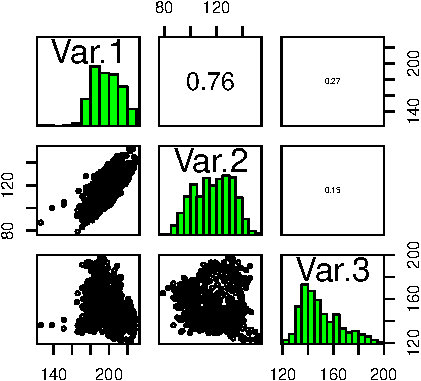
\includegraphics{Tutorial-spatstat-2_files/figure-beamer/unnamed-chunk-13-1} \end{center}
\end{frame}

\begin{frame}[fragile]{Variables \emph{compatibles}}
\protect\hypertarget{variables-compatibles}{}
Podemos incluir en el mismo modelo:

\begin{enumerate}
\tightlist
\item
  Var.1 y Var.3
\item
  Var.2 y Var.3
\end{enumerate}

Por lo tanto las fórmula polinomial

\[\log \lambda = \alpha  + \beta_1 x_1 + \beta_1' + x_1^2 + \beta_2 x_2 + \beta_2' + x_2^2 +\]

En \textbf{R}:

\begin{enumerate}
\tightlist
\item
  \texttt{\textasciitilde{}\ Var.1\ +\ Var.3\ +\ I(Var.1\^{}2)\ +\ I(Var.3\^{}2)}
\item
  \texttt{\textasciitilde{}\ Var.2\ +\ Var.3\ +\ I(Var.2\^{}2)\ +\ I(Var.3\^{}2)}
\end{enumerate}
\end{frame}

\begin{frame}[fragile]{Ajustando los modelos}
\protect\hypertarget{ajustando-los-modelos}{}
\begin{Shaded}
\begin{Highlighting}[]
\NormalTok{m1 }\OtherTok{\textless{}{-}} \FunctionTok{ppm}\NormalTok{(}\AttributeTok{Q =}\NormalTok{ puntos.}\FloatTok{2.}\NormalTok{ppp,}
          \AttributeTok{trend =} \SpecialCharTok{\textasciitilde{}}\NormalTok{ Var}\FloatTok{.1} \SpecialCharTok{+}\NormalTok{ Var}\FloatTok{.3} \SpecialCharTok{+} \FunctionTok{I}\NormalTok{(Var}\FloatTok{.1}\SpecialCharTok{\^{}}\DecValTok{2}\NormalTok{) }\SpecialCharTok{+} \FunctionTok{I}\NormalTok{(Var}\FloatTok{.3}\SpecialCharTok{\^{}}\DecValTok{2}\NormalTok{),}
          \AttributeTok{covariates =}\NormalTok{ r.im)}
\NormalTok{m2 }\OtherTok{\textless{}{-}} \FunctionTok{ppm}\NormalTok{(}\AttributeTok{Q =}\NormalTok{ puntos.}\FloatTok{2.}\NormalTok{ppp,}
          \AttributeTok{trend =} \SpecialCharTok{\textasciitilde{}}\NormalTok{ Var}\FloatTok{.2} \SpecialCharTok{+}\NormalTok{ Var}\FloatTok{.3} \SpecialCharTok{+} \FunctionTok{I}\NormalTok{(Var}\FloatTok{.2}\SpecialCharTok{\^{}}\DecValTok{2}\NormalTok{) }\SpecialCharTok{+} \FunctionTok{I}\NormalTok{(Var}\FloatTok{.3}\SpecialCharTok{\^{}}\DecValTok{2}\NormalTok{),}
          \AttributeTok{covariates =}\NormalTok{ r.im)}
\end{Highlighting}
\end{Shaded}
\end{frame}

\begin{frame}[fragile]{Comparando los modelos}
\protect\hypertarget{comparando-los-modelos}{}
\begin{Shaded}
\begin{Highlighting}[]
\FunctionTok{AIC}\NormalTok{(m1); }\FunctionTok{AIC}\NormalTok{(m2)}
\end{Highlighting}
\end{Shaded}

\begin{verbatim}
## [1] -509.172
\end{verbatim}

\begin{verbatim}
## [1] -521.2113
\end{verbatim}
\end{frame}

\begin{frame}[fragile]{Analizar los efectos estimados}
\protect\hypertarget{analizar-los-efectos-estimados}{}
\begin{Shaded}
\begin{Highlighting}[]
\NormalTok{sum.m1 }\OtherTok{\textless{}{-}} \FunctionTok{summary}\NormalTok{(m1)}
\NormalTok{knitr}\SpecialCharTok{::}\FunctionTok{kable}\NormalTok{(sum.m1}\SpecialCharTok{$}\NormalTok{coefs.SE.CI[, }\DecValTok{1}\SpecialCharTok{:}\DecValTok{5}\NormalTok{])}
\end{Highlighting}
\end{Shaded}

\begin{longtable}[]{@{}lrrrrl@{}}
\toprule\noalign{}
& Estimate & S.E. & CI95.lo & CI95.hi & Ztest \\
\midrule\noalign{}
\endhead
(Intercept) & 2.7089019 & 0.1116046 & 2.4901610 & 2.9276429 & *** \\
Var.1 & 0.1163265 & 0.0883434 & -0.0568233 & 0.2894764 & \\
Var.3 & -0.2208983 & 0.1118989 & -0.4402161 & -0.0015805 & * \\
I(Var.1\^{}2) & -0.3046825 & 0.0875528 & -0.4762828 & -0.1330821 &
*** \\
I(Var.3\^{}2) & -0.5240862 & 0.1173717 & -0.7541304 & -0.2940420 &
*** \\
\bottomrule\noalign{}
\end{longtable}
\end{frame}

\begin{frame}[fragile]{Diagnóstico - Residuales}
\protect\hypertarget{diagnuxf3stico---residuales}{}
\begin{Shaded}
\begin{Highlighting}[]
\FunctionTok{par}\NormalTok{(}\AttributeTok{mar =} \FunctionTok{c}\NormalTok{(}\DecValTok{2}\NormalTok{,}\DecValTok{2}\NormalTok{,}\DecValTok{2}\NormalTok{,}\DecValTok{2}\NormalTok{))}
\FunctionTok{diagnose.ppm}\NormalTok{(m1, }\AttributeTok{main =} \StringTok{""}\NormalTok{, }\AttributeTok{cex.axis =} \FloatTok{0.25}\NormalTok{)}
\end{Highlighting}
\end{Shaded}

\begin{center}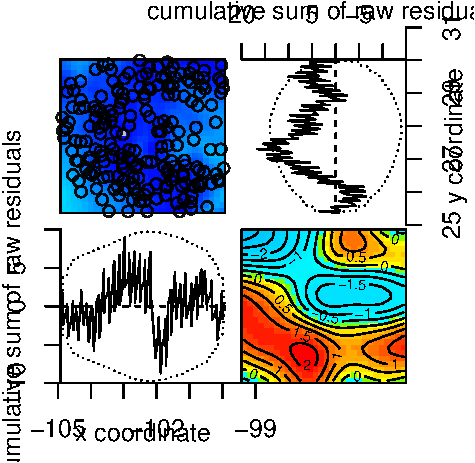
\includegraphics{Tutorial-spatstat-2_files/figure-beamer/unnamed-chunk-17-1} \end{center}
\end{frame}

\begin{frame}[fragile]{Diangnóstico - Residuales}
\protect\hypertarget{diangnuxf3stico---residuales}{}
\begin{Shaded}
\begin{Highlighting}[]
\FunctionTok{par}\NormalTok{(}\AttributeTok{mar =} \FunctionTok{c}\NormalTok{(}\DecValTok{2}\NormalTok{,}\DecValTok{2}\NormalTok{,}\DecValTok{2}\NormalTok{,}\DecValTok{2}\NormalTok{))}
\FunctionTok{diagnose.ppm}\NormalTok{(m2, }\AttributeTok{main =} \StringTok{""}\NormalTok{, }\AttributeTok{cex.axis =} \FloatTok{0.25}\NormalTok{)}
\end{Highlighting}
\end{Shaded}

\begin{center}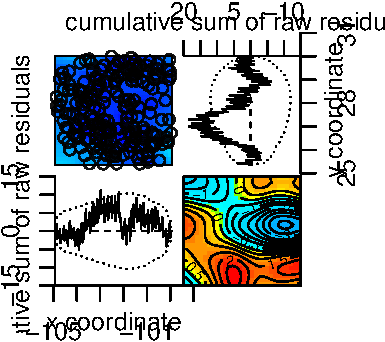
\includegraphics{Tutorial-spatstat-2_files/figure-beamer/unnamed-chunk-18-1} \end{center}
\end{frame}

\begin{frame}[fragile]{Diagnóstico - Ripley}
\protect\hypertarget{diagnuxf3stico---ripley}{}
\begin{Shaded}
\begin{Highlighting}[]
\NormalTok{K1 }\OtherTok{\textless{}{-}} \FunctionTok{envelope}\NormalTok{(m1, }\AttributeTok{fun =}\NormalTok{ Kest, }\AttributeTok{nsim =} \DecValTok{39}\NormalTok{)}
\end{Highlighting}
\end{Shaded}

\begin{verbatim}
## Generating 39 simulated realisations of fitted Poisson model  ...
## 1, 2, 3, 4, 5, 6, 7, 8, 9, 10, 11, 12, 13, 14, 15, 16, 17, 18, 19, 20,
## 21, 22, 23, 24, 25, 26, 27, 28, 29, 30, 31, 32, 33, 34, 35, 36, 37, 38, 
## 39.
## 
## Done.
\end{verbatim}

\begin{Shaded}
\begin{Highlighting}[]
\NormalTok{K2 }\OtherTok{\textless{}{-}} \FunctionTok{envelope}\NormalTok{(m2, }\AttributeTok{fun =}\NormalTok{ Kest, }\AttributeTok{nsim =} \DecValTok{39}\NormalTok{)}
\end{Highlighting}
\end{Shaded}

\begin{verbatim}
## Generating 39 simulated realisations of fitted Poisson model  ...
## 1, 2, 3, 4, 5, 6, 7, 8, 9, 10, 11, 12, 13, 14, 15, 16, 17, 18, 19, 20,
## 21, 22, 23, 24, 25, 26, 27, 28, 29, 30, 31, 32, 33, 34, 35, 36, 37, 38, 
## 39.
## 
## Done.
\end{verbatim}
\end{frame}

\begin{frame}[fragile]{Diagnóstico - Ripley}
\protect\hypertarget{diagnuxf3stico---ripley-1}{}
\begin{Shaded}
\begin{Highlighting}[]
\FunctionTok{plot}\NormalTok{(K1, }\AttributeTok{cex =} \FloatTok{0.5}\NormalTok{)}
\end{Highlighting}
\end{Shaded}

\begin{center}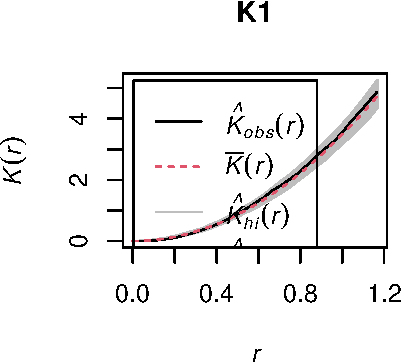
\includegraphics{Tutorial-spatstat-2_files/figure-beamer/unnamed-chunk-20-1} \end{center}
\end{frame}

\begin{frame}[fragile]{Diangóstico - Ripley}
\protect\hypertarget{dianguxf3stico---ripley}{}
\begin{Shaded}
\begin{Highlighting}[]
\FunctionTok{plot}\NormalTok{(K2, }\AttributeTok{cex =} \FloatTok{0.5}\NormalTok{)}
\end{Highlighting}
\end{Shaded}

\begin{center}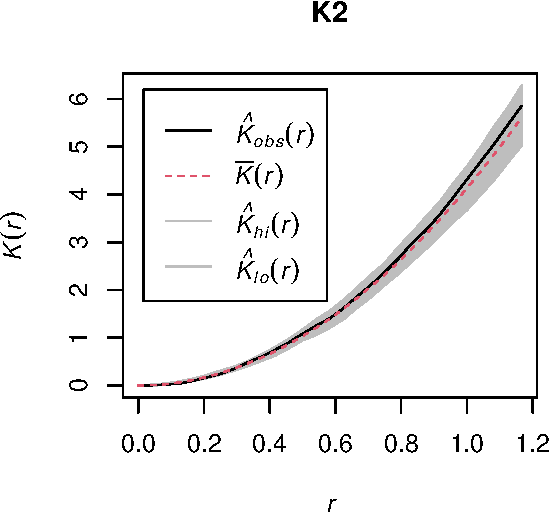
\includegraphics{Tutorial-spatstat-2_files/figure-beamer/unnamed-chunk-21-1} \end{center}
\end{frame}

\begin{frame}[fragile]{Resumen del análisis}
\protect\hypertarget{resumen-del-anuxe1lisis}{}
\begin{itemize}
\item
  AIC menor para \texttt{m1}
\item
  Residuales dentro de tolerancia para \texttt{m1}
\item
  Prueba de ripley correcta para ambos modelos

  \begin{itemize}
  \tightlist
  \item
    No parece necesario modelar autocorrelación (lo haremos a
    continuación)
  \end{itemize}
\item
  Evidencia \emph{favorece} a \texttt{m1}
\end{itemize}
\end{frame}

\begin{frame}[fragile]{Revisando la predicción}
\protect\hypertarget{revisando-la-predicciuxf3n}{}
\begin{Shaded}
\begin{Highlighting}[]
\FunctionTok{plot}\NormalTok{(m1, }\AttributeTok{se =}\NormalTok{ F, }\AttributeTok{main =} \StringTok{""}\NormalTok{)}
\end{Highlighting}
\end{Shaded}

\begin{center}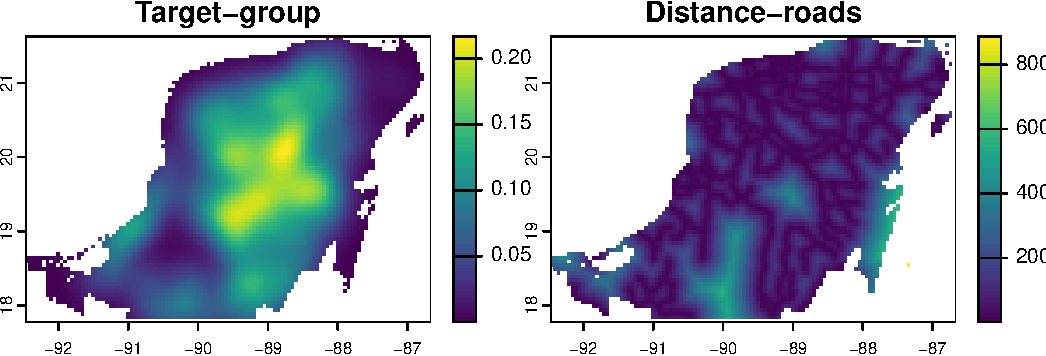
\includegraphics{Tutorial-spatstat-2_files/figure-beamer/unnamed-chunk-22-1} \end{center}
\end{frame}

\begin{frame}[fragile]{Guardando los resultados}
\protect\hypertarget{guardando-los-resultados}{}
\begin{Shaded}
\begin{Highlighting}[]
\NormalTok{pred }\OtherTok{\textless{}{-}} \FunctionTok{predict}\NormalTok{(m1)}
\NormalTok{pred.r }\OtherTok{\textless{}{-}} \FunctionTok{rast}\NormalTok{(pred)}
\FunctionTok{writeRaster}\NormalTok{(pred.r, }\StringTok{"Predicción{-}m1.tif"}\NormalTok{,}
            \AttributeTok{overwrite =}\NormalTok{ T)}
\end{Highlighting}
\end{Shaded}
\end{frame}

\hypertarget{modelando-los-efectos-espaciales}{%
\section{Modelando los efectos
espaciales}\label{modelando-los-efectos-espaciales}}

\begin{frame}{Modelos de interacción}
\protect\hypertarget{modelos-de-interacciuxf3n}{}
\begin{itemize}
\tightlist
\item
  Estiman efecto aleatorio para puntos cercanos
\item
  Sirven para procesos de exclusión o agregación moderada
\item
  Hay varios tipos de interacciones entre puntos
\end{itemize}
\end{frame}

\begin{frame}{¿Qué es interacción?}
\protect\hypertarget{quuxe9-es-interacciuxf3n}{}
\begin{center}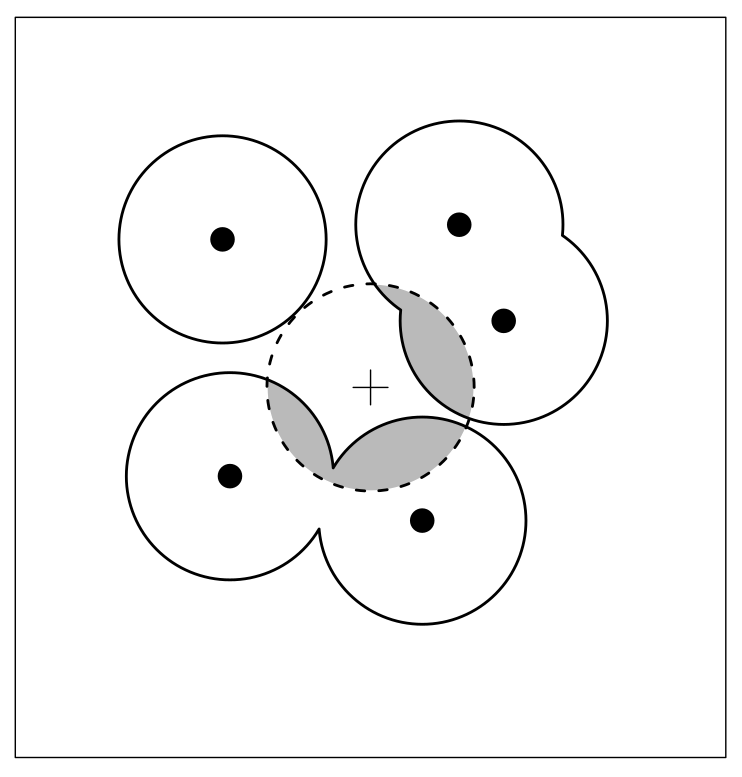
\includegraphics[width=10.31in]{Figuras/Interaccion-puntos} \end{center}
\end{frame}

\begin{frame}{Tipos de interacciones}
\protect\hypertarget{tipos-de-interacciones}{}
\begin{figure}

{\centering 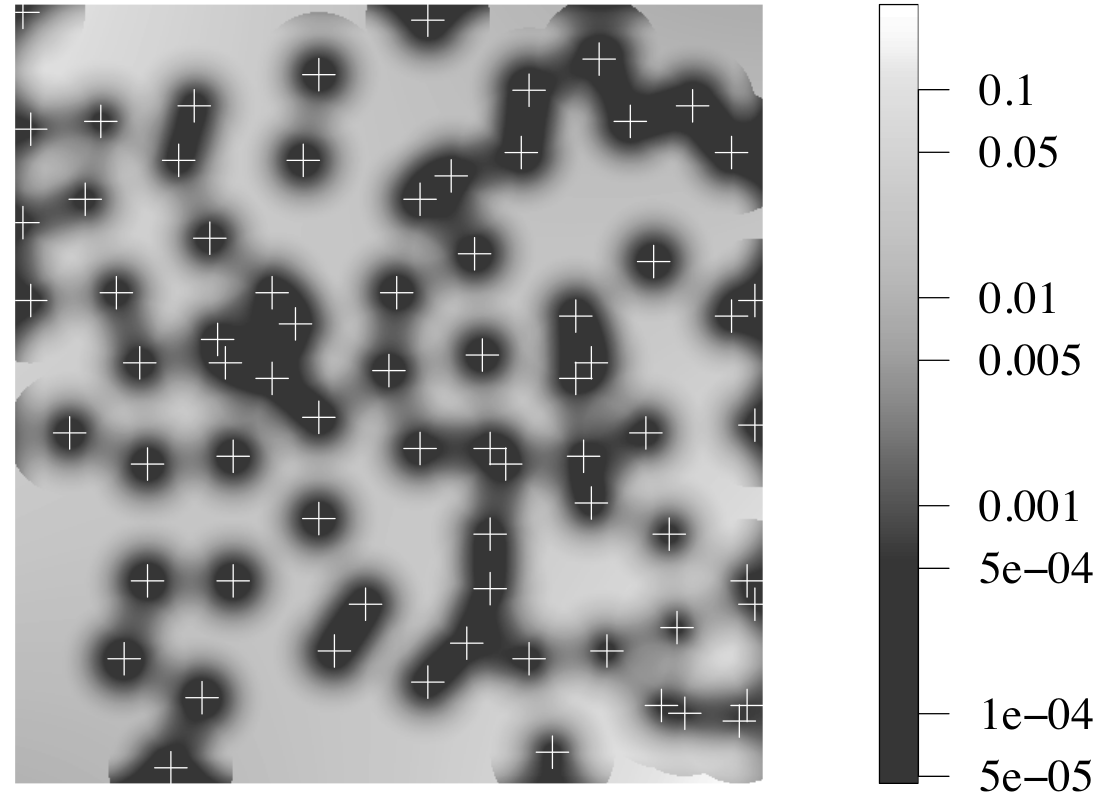
\includegraphics[width=15.29in]{Figuras/Tipos-interacciones} 

}

\caption{Crédito a Baddeley et al (2016)}\label{fig:unnamed-chunk-25}
\end{figure}
\end{frame}

\begin{frame}{Modelos de interacción en \texttt{spatstat}}
\protect\hypertarget{modelos-de-interacciuxf3n-en-spatstat}{}
\begin{center}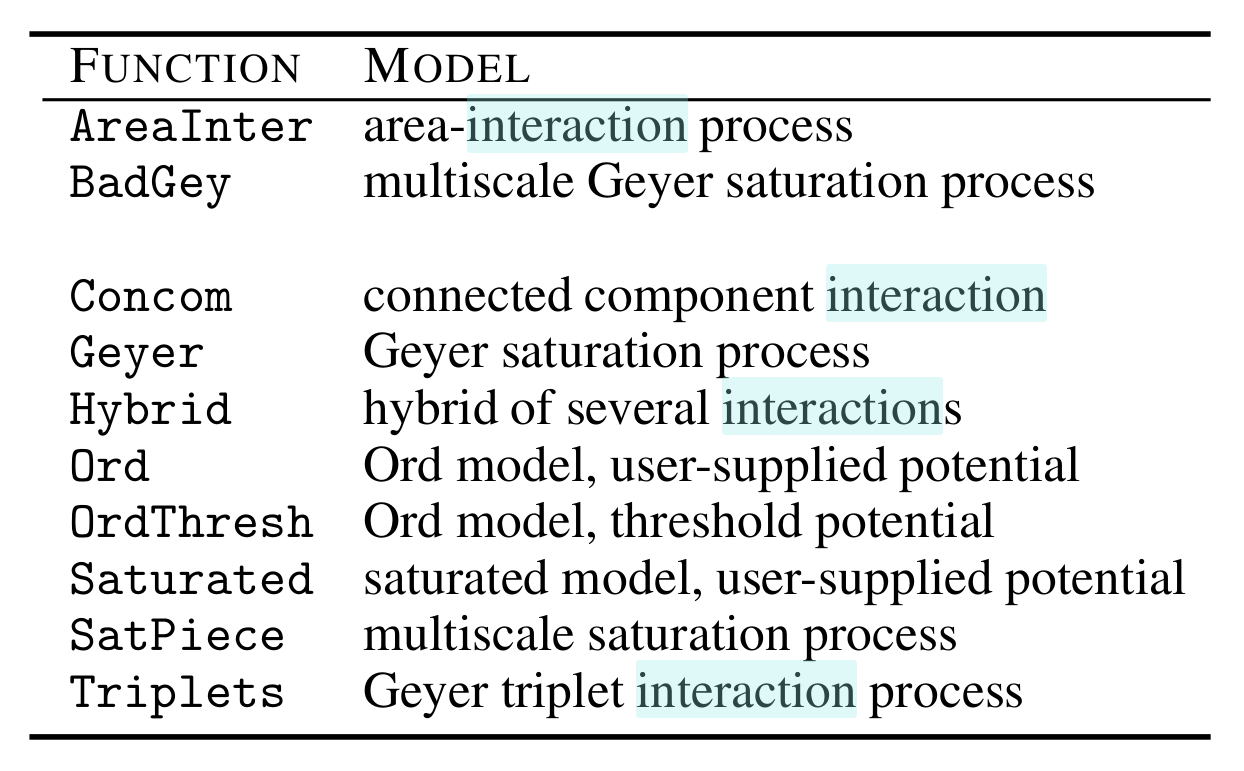
\includegraphics[width=17.28in]{Figuras/Tabla-tipos-interacciones} \end{center}
\end{frame}

\begin{frame}[fragile]{Para generar un modelo de interacción}
\protect\hypertarget{para-generar-un-modelo-de-interacciuxf3n}{}
\begin{enumerate}
\tightlist
\item
  Establecer tamaño del búfer
\end{enumerate}

\begin{Shaded}
\begin{Highlighting}[]
\NormalTok{rr }\OtherTok{\textless{}{-}} \FunctionTok{data.frame}\NormalTok{(}\AttributeTok{r=}\FunctionTok{seq}\NormalTok{(}\DecValTok{1}\NormalTok{,}\DecValTok{5}\NormalTok{,}\AttributeTok{by=}\DecValTok{1}\NormalTok{))}
\NormalTok{p }\OtherTok{\textless{}{-}} \FunctionTok{profilepl}\NormalTok{(rr, Strauss, }
\NormalTok{               puntos.}\FloatTok{2.}\NormalTok{ppp }\SpecialCharTok{\textasciitilde{}}\NormalTok{ Var}\FloatTok{.1} \SpecialCharTok{+}\NormalTok{ Var}\FloatTok{.3} \SpecialCharTok{+} \FunctionTok{I}\NormalTok{(Var}\FloatTok{.1}\SpecialCharTok{\^{}}\DecValTok{2}\NormalTok{) }\SpecialCharTok{+} \FunctionTok{I}\NormalTok{(Var}\FloatTok{.3}\SpecialCharTok{\^{}}\DecValTok{2}\NormalTok{),}
          \AttributeTok{covariates =}\NormalTok{ r.im, }\AttributeTok{aic=}\NormalTok{F, }\AttributeTok{rbord =} \FloatTok{0.1}\NormalTok{)}
\end{Highlighting}
\end{Shaded}

\begin{verbatim}
## comparing 5 models...
\end{verbatim}

\begin{verbatim}
## 1, 2, 3, 4, 
## 5.
\end{verbatim}

\begin{verbatim}
## fitting optimal model...
\end{verbatim}

\begin{verbatim}
## done.
\end{verbatim}
\end{frame}

\begin{frame}[fragile]{Para generar un modelo de interacción}
\protect\hypertarget{para-generar-un-modelo-de-interacciuxf3n-1}{}
\begin{Shaded}
\begin{Highlighting}[]
\FunctionTok{plot}\NormalTok{(p, }\AttributeTok{main =} \StringTok{""}\NormalTok{)}
\end{Highlighting}
\end{Shaded}

\begin{center}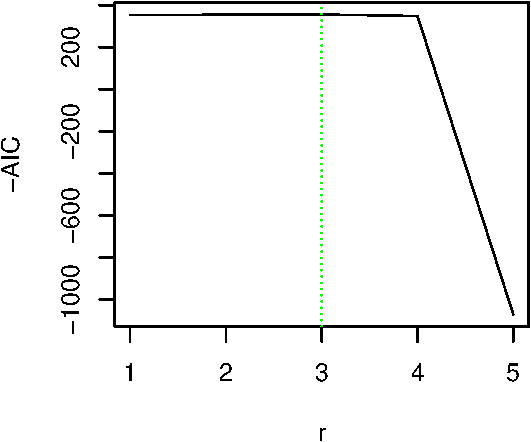
\includegraphics{Tutorial-spatstat-2_files/figure-beamer/unnamed-chunk-28-1} \end{center}
\end{frame}

\begin{frame}[fragile]{Para generar un modelo de interacción}
\protect\hypertarget{para-generar-un-modelo-de-interacciuxf3n-2}{}
Un radio de tamaño 2 minimiza la pseudo-verosimilitud, de modo que el
modelo de interacción con la fórmula de m1 es:

\begin{Shaded}
\begin{Highlighting}[]
\NormalTok{m1.int }\OtherTok{\textless{}{-}} \FunctionTok{ppm}\NormalTok{(}\AttributeTok{Q =}\NormalTok{ puntos.}\FloatTok{2.}\NormalTok{ppp,}
          \AttributeTok{trend =} \SpecialCharTok{\textasciitilde{}}\NormalTok{ Var}\FloatTok{.2} \SpecialCharTok{+}\NormalTok{ Var}\FloatTok{.3} \SpecialCharTok{+} \FunctionTok{I}\NormalTok{(Var}\FloatTok{.2}\SpecialCharTok{\^{}}\DecValTok{2}\NormalTok{) }\SpecialCharTok{+} \FunctionTok{I}\NormalTok{(Var}\FloatTok{.3}\SpecialCharTok{\^{}}\DecValTok{2}\NormalTok{),}
          \AttributeTok{covariates =}\NormalTok{ r.im,}
          \FunctionTok{AreaInter}\NormalTok{(rr}\SpecialCharTok{$}\NormalTok{r[p}\SpecialCharTok{$}\NormalTok{iopt]), }\AttributeTok{rbord =} \FloatTok{0.1}\NormalTok{) }\CommentTok{\#Interacción}
\end{Highlighting}
\end{Shaded}
\end{frame}

\begin{frame}[fragile]{Efectos estimados}
\protect\hypertarget{efectos-estimados}{}
\begin{Shaded}
\begin{Highlighting}[]
\NormalTok{sum.int }\OtherTok{\textless{}{-}} \FunctionTok{summary}\NormalTok{(m1.int)}
\NormalTok{knitr}\SpecialCharTok{::}\FunctionTok{kable}\NormalTok{(sum.int}\SpecialCharTok{$}\NormalTok{coefs.SE.CI[, }\DecValTok{1}\SpecialCharTok{:}\DecValTok{4}\NormalTok{])}
\end{Highlighting}
\end{Shaded}
\end{frame}

\begin{frame}[fragile]{Efectos estimados - comparación}
\protect\hypertarget{efectos-estimados---comparaciuxf3n}{}
\begin{Shaded}
\begin{Highlighting}[]
\FunctionTok{coef}\NormalTok{(m1)}
\end{Highlighting}
\end{Shaded}

\begin{verbatim}
## (Intercept)       Var.1       Var.3  I(Var.1^2)  I(Var.3^2) 
##   2.7089019   0.1163265  -0.2208983  -0.3046825  -0.5240862
\end{verbatim}

\begin{Shaded}
\begin{Highlighting}[]
\FunctionTok{coef}\NormalTok{(m1.int)}
\end{Highlighting}
\end{Shaded}

\begin{verbatim}
## (Intercept)       Var.2       Var.3  I(Var.2^2)  I(Var.3^2) Interaction 
##  2.87549775  0.08478505 -0.00164637 -0.42014097 -0.52671442          NA
\end{verbatim}
\end{frame}

\begin{frame}[fragile]{Diangóstico}
\protect\hypertarget{dianguxf3stico}{}
\begin{Shaded}
\begin{Highlighting}[]
\NormalTok{K.int }\OtherTok{\textless{}{-}} \FunctionTok{envelope}\NormalTok{(m1.int, Kest, }\AttributeTok{nsim =} \DecValTok{39}\NormalTok{)}
\end{Highlighting}
\end{Shaded}

\begin{verbatim}
## Generating 39 simulated realisations of fitted Gibbs model  ...
## 1, 2, 3, 4, 5, 6, 7, 8, 9, 10, 11, 12, 13, 14, 15, 16, 17, 18, 19, 20,
## 21, 22, 23, 24, 25, 26, 27, 28, 29, 30, 31, 32, 33, 34, 35, 36, 37, 38, 
## 39.
## 
## Done.
\end{verbatim}
\end{frame}

\begin{frame}[fragile]{Diangóstico}
\protect\hypertarget{dianguxf3stico-1}{}
\begin{Shaded}
\begin{Highlighting}[]
\FunctionTok{plot}\NormalTok{(K.int)}
\end{Highlighting}
\end{Shaded}

\begin{center}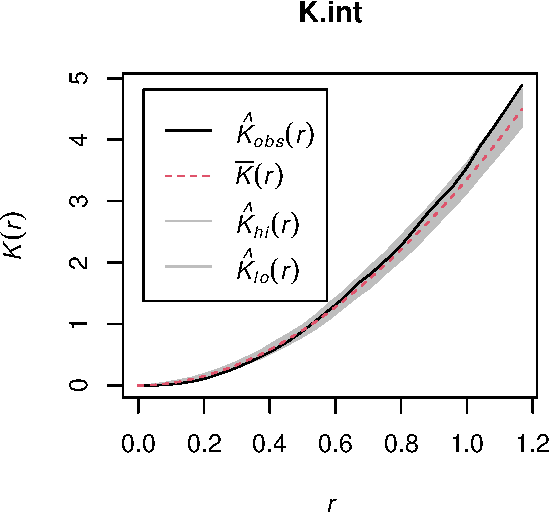
\includegraphics{Tutorial-spatstat-2_files/figure-beamer/unnamed-chunk-33-1} \end{center}
\end{frame}

\begin{frame}{Favorabilidad}
\protect\hypertarget{favorabilidad}{}
\begin{center}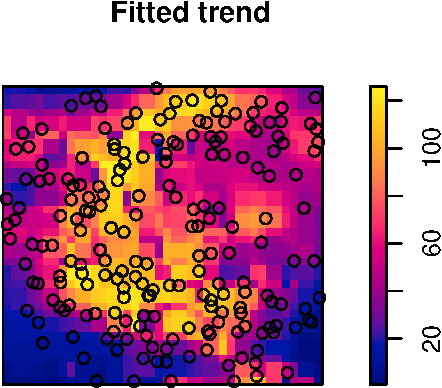
\includegraphics{Tutorial-spatstat-2_files/figure-beamer/unnamed-chunk-34-1} \end{center}
\end{frame}

\hypertarget{proceso-cox-log-gaussiano}{%
\section{Proceso Cox log-Gaussiano}\label{proceso-cox-log-gaussiano}}

\begin{frame}{¿Qué es?}
\protect\hypertarget{quuxe9-es}{}
\begin{itemize}
\item
  En MPPs

  \begin{itemize}
  \tightlist
  \item
    Intensidad es explicada por covariables si
  \item
    Covariables rara vez explican puntos agregados
  \end{itemize}
\item
  Gaussiano = Distribución normal

  \begin{itemize}
  \tightlist
  \item
    Efecto aleatorio con distribución normal multivariada
  \end{itemize}
\end{itemize}
\end{frame}

\begin{frame}{¿Qué es?}
\protect\hypertarget{quuxe9-es-1}{}
\[\log \lambda_i = \alpha + \beta_1 x_{1,i} + \dots + G(u_i, v_i)\] -
\(\alpha\) es el intercepto global - \(G(u_i)\) es el intercepto
aleatorio para cada píxel - Cuando todas las \(x = 0\), la intensidad en
el píxel \(i\) es \(\exp(\alpha + G(u_i))\)
\end{frame}

\begin{frame}[fragile]{¿Con qué se ajusta un LGCP en \textbf{R}?}
\protect\hypertarget{con-quuxe9-se-ajusta-un-lgcp-en-r}{}
\begin{itemize}
\item
  Frecuentista - \texttt{spatstat} (rápido poco preciso)
\item
  Bayesiano

  \begin{itemize}
  \tightlist
  \item
    \texttt{RINLA} (moderadamente rápido, moderadamente preciso)
  \item
    \texttt{lgcp} (muuuuy lento, bastante preciso)
  \end{itemize}
\item
  Frecuentista son aproximaciones, y Bayesiano son estimaciones
  \emph{verdaderas}
\end{itemize}
\end{frame}

\begin{frame}[fragile]{Ajustando un LGCP con \texttt{spatstat}}
\protect\hypertarget{ajustando-un-lgcp-con-spatstat}{}
\begin{Shaded}
\begin{Highlighting}[]
\NormalTok{m1.lgcp }\OtherTok{\textless{}{-}} \FunctionTok{kppm}\NormalTok{(puntos.}\FloatTok{2.}\NormalTok{ppp,}
                \AttributeTok{trend =} \SpecialCharTok{\textasciitilde{}}\NormalTok{ Var}\FloatTok{.2} \SpecialCharTok{+}\NormalTok{ Var}\FloatTok{.3} \SpecialCharTok{+} \FunctionTok{I}\NormalTok{(Var}\FloatTok{.2}\SpecialCharTok{\^{}}\DecValTok{2}\NormalTok{) }\SpecialCharTok{+} \FunctionTok{I}\NormalTok{(Var}\FloatTok{.3}\SpecialCharTok{\^{}}\DecValTok{2}\NormalTok{),}
                \AttributeTok{covariates =}\NormalTok{ r.im,}
                \AttributeTok{clusters =} \StringTok{"LGCP"}\NormalTok{,}
                \AttributeTok{statistic =} \StringTok{"K"}\NormalTok{, }\CommentTok{\# K de Ripley}
                \AttributeTok{method =} \StringTok{"mincon"}\NormalTok{) }\CommentTok{\# Modelo de varianza}
\end{Highlighting}
\end{Shaded}
\end{frame}

\begin{frame}[fragile]{Ajustando un LGCP con \texttt{spatstat}}
\protect\hypertarget{ajustando-un-lgcp-con-spatstat-1}{}
\begin{Shaded}
\begin{Highlighting}[]
\NormalTok{sum.lgcp }\OtherTok{\textless{}{-}} \FunctionTok{summary}\NormalTok{(m1.lgcp)}
\NormalTok{knitr}\SpecialCharTok{::}\FunctionTok{kable}\NormalTok{(sum.lgcp}\SpecialCharTok{$}\NormalTok{coefs.SE.CI[, }\DecValTok{1}\SpecialCharTok{:}\DecValTok{4}\NormalTok{])}
\end{Highlighting}
\end{Shaded}

\begin{longtable}[]{@{}lrrrr@{}}
\toprule\noalign{}
& Estimate & S.E. & CI95.lo & CI95.hi \\
\midrule\noalign{}
\endhead
(Intercept) & 2.8710581 & 0.3194624 & 2.2449234 & 3.4971929 \\
Var.2 & 0.1113775 & 0.0921967 & -0.0693247 & 0.2920797 \\
Var.3 & 0.0049808 & 0.1157026 & -0.2217922 & 0.2317538 \\
I(Var.2\^{}2) & -0.4756438 & 0.1028281 & -0.6771832 & -0.2741044 \\
I(Var.3\^{}2) & -0.5258717 & 0.1119727 & -0.7453342 & -0.3064093 \\
\bottomrule\noalign{}
\end{longtable}
\end{frame}

\begin{frame}[fragile]{Comparando con MPP}
\protect\hypertarget{comparando-con-mpp}{}
\begin{Shaded}
\begin{Highlighting}[]
\NormalTok{knitr}\SpecialCharTok{::}\FunctionTok{kable}\NormalTok{(sum.m1}\SpecialCharTok{$}\NormalTok{coefs.SE.CI[, }\FunctionTok{c}\NormalTok{(}\DecValTok{1}\NormalTok{, }\DecValTok{2}\NormalTok{, }\DecValTok{3}\NormalTok{, }\DecValTok{4}\NormalTok{)])}
\end{Highlighting}
\end{Shaded}

\begin{longtable}[]{@{}lrrrr@{}}
\toprule\noalign{}
& Estimate & S.E. & CI95.lo & CI95.hi \\
\midrule\noalign{}
\endhead
(Intercept) & 2.7089019 & 0.1116046 & 2.4901610 & 2.9276429 \\
Var.1 & 0.1163265 & 0.0883434 & -0.0568233 & 0.2894764 \\
Var.3 & -0.2208983 & 0.1118989 & -0.4402161 & -0.0015805 \\
I(Var.1\^{}2) & -0.3046825 & 0.0875528 & -0.4762828 & -0.1330821 \\
I(Var.3\^{}2) & -0.5240862 & 0.1173717 & -0.7541304 & -0.2940420 \\
\bottomrule\noalign{}
\end{longtable}
\end{frame}

\begin{frame}[fragile]{Predicciones}
\protect\hypertarget{predicciones}{}
\begin{Shaded}
\begin{Highlighting}[]
\FunctionTok{par}\NormalTok{(}\AttributeTok{mfrow =} \FunctionTok{c}\NormalTok{(}\DecValTok{1}\NormalTok{, }\DecValTok{3}\NormalTok{))}
\FunctionTok{plot}\NormalTok{(m2, }\AttributeTok{se =}\NormalTok{ F, }\AttributeTok{trend =}\NormalTok{ T, }\AttributeTok{main =} \StringTok{"Poisson"}\NormalTok{)}
\FunctionTok{plot}\NormalTok{(m1.int, }\AttributeTok{se =}\NormalTok{ F, }\AttributeTok{trend =}\NormalTok{ T, }\AttributeTok{cif =}\NormalTok{ F, }\AttributeTok{main =} \StringTok{"Interacción"}\NormalTok{)}
\FunctionTok{plot}\NormalTok{(m1.lgcp, }\AttributeTok{what =} \StringTok{"intensity"}\NormalTok{, }\AttributeTok{main =} \StringTok{"LGCP"}\NormalTok{)}
\end{Highlighting}
\end{Shaded}

\begin{center}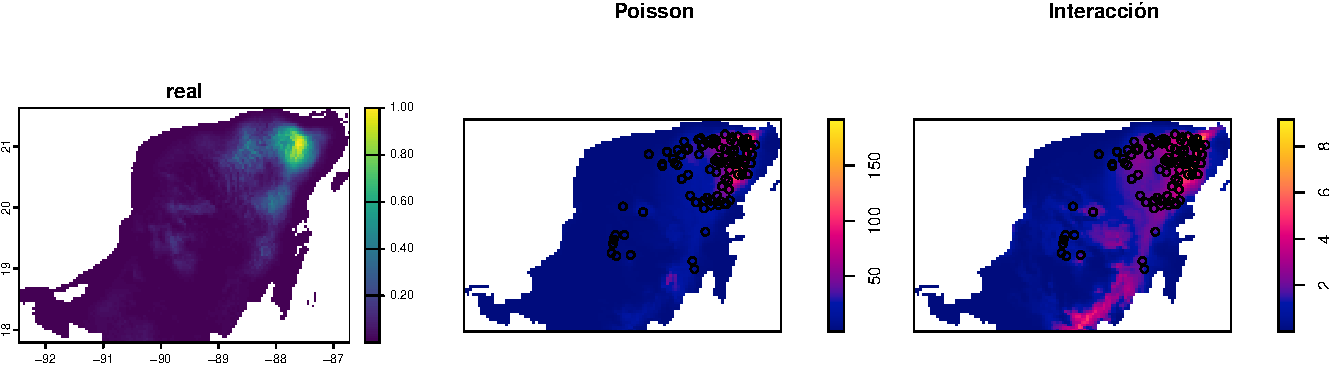
\includegraphics{Tutorial-spatstat-2_files/figure-beamer/unnamed-chunk-38-1} \end{center}
\end{frame}

\begin{frame}[fragile]{Diagnóstico}
\protect\hypertarget{diagnuxf3stico}{}
\begin{Shaded}
\begin{Highlighting}[]
\NormalTok{K.lgcp }\OtherTok{\textless{}{-}} \FunctionTok{envelope}\NormalTok{(m1.lgcp, Kest, }\AttributeTok{nsim =} \DecValTok{39}\NormalTok{)}
\end{Highlighting}
\end{Shaded}

\begin{verbatim}
## Generating 39 simulated realisations of fitted cluster model  ...
## 1, 2, 3, 4, 5, 6, 7, 8, 9, 10, 11, 12, 13, 14, 15, 16, 17, 18, 19, 20,
## 21, 22, 23, 24, 25, 26, 27, 28, 29, 30, 31, 32, 33, 34, 35, 36, 37, 38, 
## 39.
## 
## Done.
\end{verbatim}
\end{frame}

\begin{frame}[fragile]{Diangóstico}
\protect\hypertarget{dianguxf3stico-2}{}
\begin{Shaded}
\begin{Highlighting}[]
\FunctionTok{plot}\NormalTok{(K.lgcp)}
\end{Highlighting}
\end{Shaded}

\begin{center}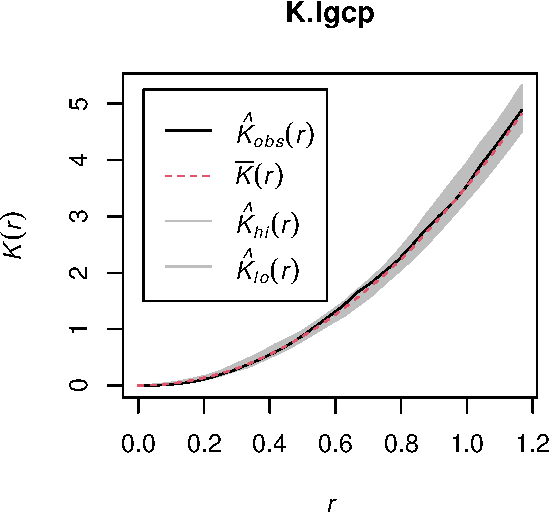
\includegraphics{Tutorial-spatstat-2_files/figure-beamer/unnamed-chunk-40-1} \end{center}
\end{frame}

\begin{frame}[fragile]{Conclusiones}
\protect\hypertarget{conclusiones}{}
\begin{itemize}
\item
  Modelo Poisson

  \begin{itemize}
  \tightlist
  \item
    Más simple, y no parece tener problemas
  \item
    IC de estimaciones más amplios que LGCP
  \end{itemize}
\item
  Interacción

  \begin{itemize}
  \tightlist
  \item
    IC más amplios que MPP
  \end{itemize}
\item
  LGCP

  \begin{itemize}
  \tightlist
  \item
    Función K más cercana a expectativa teórica \#\#\# Alternativas de
    modelación
  \end{itemize}
\item
  Respuestas bisagra: Regresión por partes
\item
  Respuestas no lineales: Suavizadores GAM
\item
  Interacciones entre variables
\item
  LASSO con paquete \texttt{ppmlasso} (Warton y Renner 2013)
\end{itemize}
\end{frame}

\end{document}
